
\subsection{Kiểm thử các xử lý logic phía máy chủ}

Để đảm bảo các chức năng cốt lõi của hệ thống hoạt động chính xác, backend được kiểm thử với 2 phương pháp chính: kiểm thử đơn vị (unit testing) cho các hàm và module xử lý nghiệp vụ riêng lẻ, và kiểm thử tích hợp API (API integration testing) để xác minh sự tương tác giữa các thành phần và tính đúng đắn của các điểm cuối (endpoints) mà ứng dụng di động sẽ giao tiếp.

\subsubsection{Kiểm thử đơn vị}

\textbf{Phạm vi kiểm thử}

\noindent Phạm vi kiểm thử đơn vị của ứng dụng VieVu bao gồm kiểm thử các hàm xử lý và model của server Backend Python với FastAPI. 

\noindent
\textbf{Môi trường kiểm thử}

\noindent Môi trường kiểm thử đơn vị được thiết lập bằng cách sử dụng \texttt{pytest}~\cite{pytest}, một framework kiểm thử phổ biến, mạnh mẽ và linh hoạt cho Python. \texttt{pytest} cung cấp nhiều tính năng nâng cao và cũng có khả năng khám phá và chạy các kiểm thử được viết bằng thư viện \texttt{unittest} tích hợp sẵn của Python. Trong dự án này, \texttt{pytest} được sử dụng để xác minh tính đúng đắn của các hàm xử lý logic cho những chức năng cốt lõi như gợi ý địa điểm, tổng hợp lịch trình từ tin nhắn và chức năng tìm kiếm tổng hợp của ứng dụng.

\noindent
\textbf{Kết quả kiểm thử}
% Độ phủ nhánh cho các hàm xử lý logic của server labeling ảnh được miêu tả như
% Hình 4.17 và đạt 100%, với phạm vi kiểm thử bao gồm các hàm xử lý chính như
% resize ảnh, phân nhóm khuôn mặt và các hàm xử lý của model AI. Đối với server
% tạo video, độ phủ nhánh được miêu tả như Hình 4.18 và đạt 92.59%, với phạm vi
% 61
% kiểm thử bao gồm các hàm xử lý chính như tạo kịch bản video và tạo kịch bản cho
% video
\noindent Độ phủ và kết quả kiểm thử xử lý logic được trình bày trong Hình \ref{fig:pytest-testing}. Hệ thống đã được kiểm thử với tổng cộng 513 câu lệnh và đạt độ phủ 94\%, với phạm vi kiểm thử bao gồm hầu hết các module và hàm xử lý chính như gợi ý, tổng hợp lịch trình, phân loại và nhận diện. Ngoài ra các hàm tạo route API, tiền xử lý dữ liệu và xác thực người dùng tại server backend cũng dược kiểm thử đầy đủ với độ phủ xấp xỉ 90\%.

\begin{figure}[H]
    \centering  
    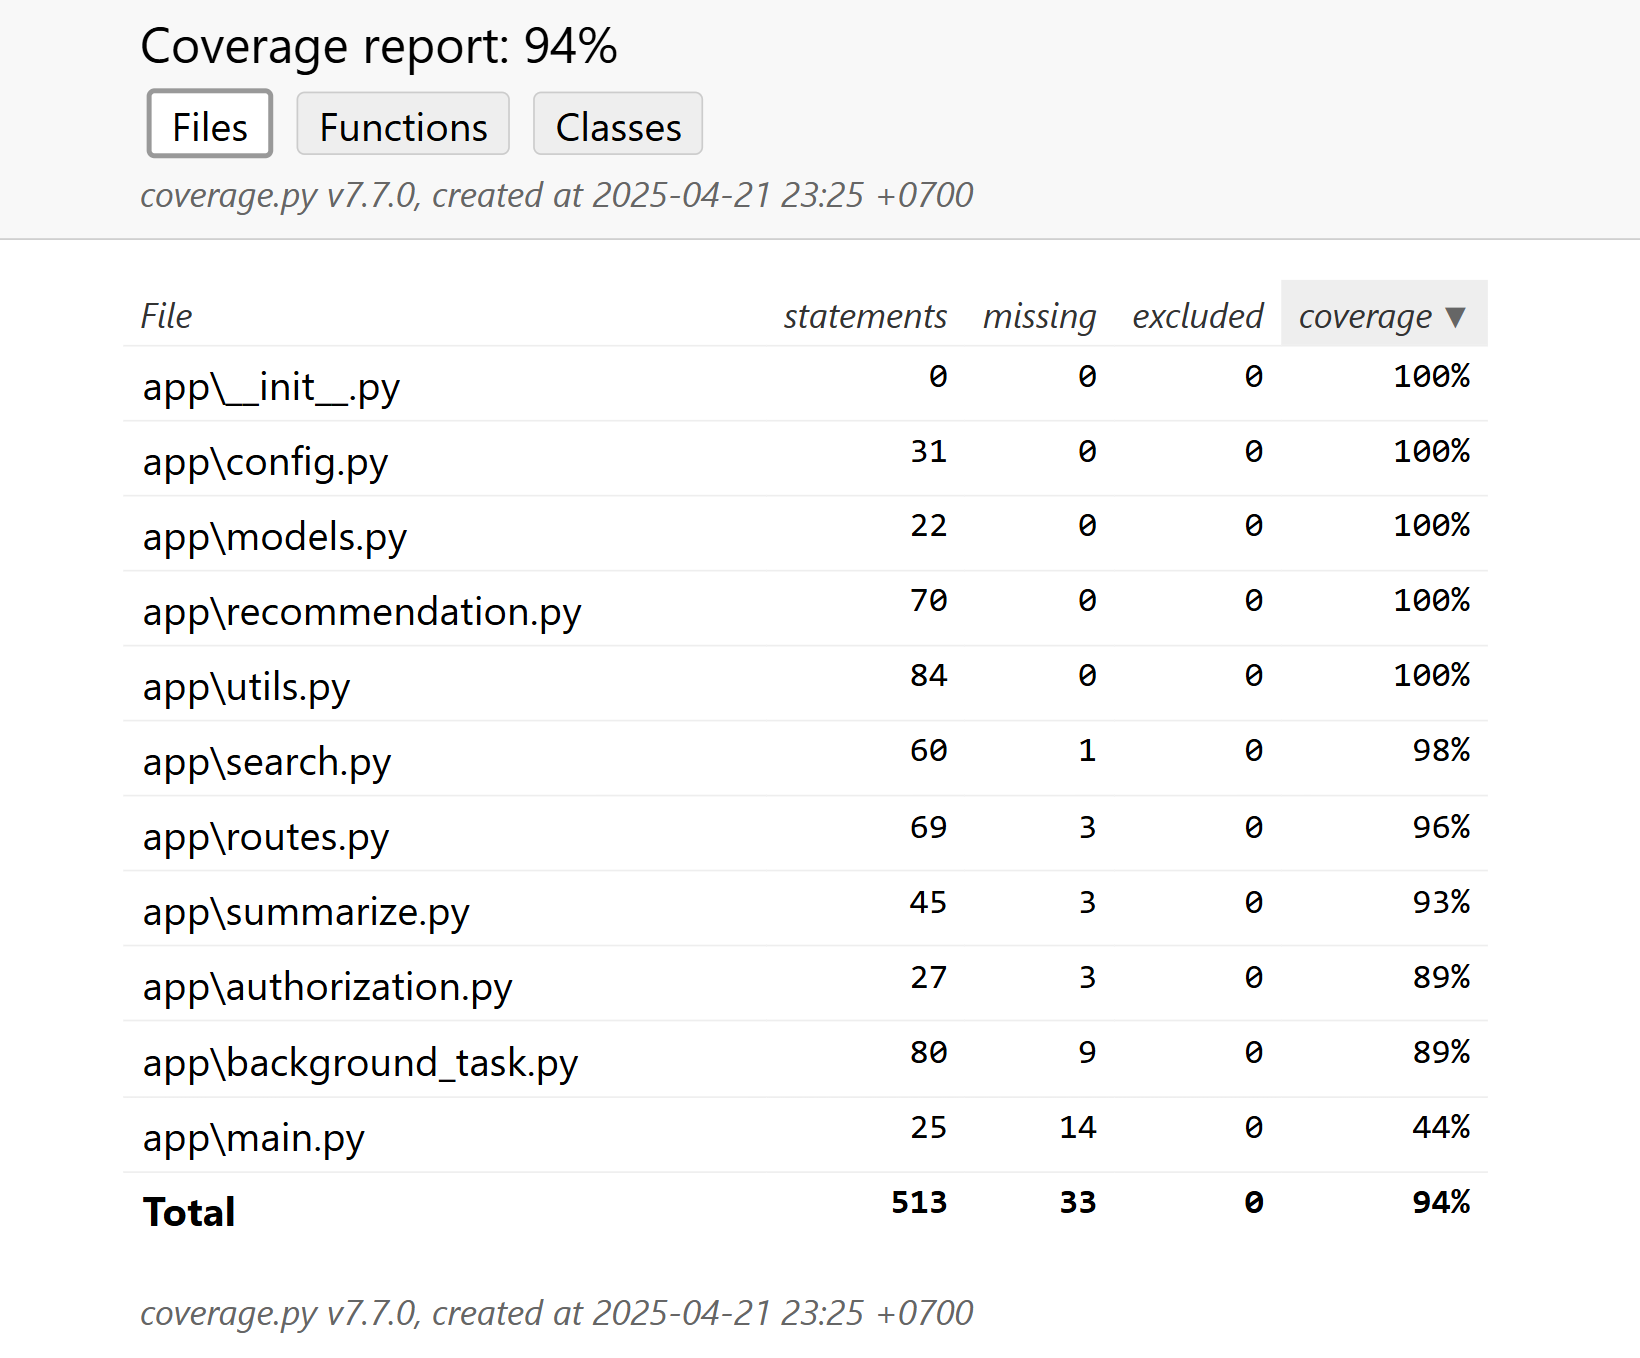
\includegraphics[width=0.8\textwidth]{figures/c4/unittest.png}
    \caption{Độ phủ kiểm thử xử lý logic với Pytest.}
    \label{fig:pytest-testing}
\end{figure}


\subsubsection{Kiểm thử API}

Chi tiết các ca kiểm thử (miêu tả, input và output) được mô tả dưới Bảng \ref{tab:api-test-cases}. Hình \ref{fig:postman} dưới đây mô tả các API endpoint được kiểm thử với Postman~\cite{postman}.  
% Bảng 4.2 mô tả một số kịch bảng kiểm thử API chính cho ứng dụng. 

\small
\begin{xltabular}{\textwidth}{|c|p{2cm}|X|X|c|}
    \caption{Các kịch bản kiểm thử API chính} \label{tab:api-test-cases} \\
    \hline
    \textbf{STT} & \textbf{API} & \textbf{Ca kiểm thử} & \textbf{Kết quả kỳ vọng} & \textbf{Tình trạng} \\
    \hline
    \endfirsthead
    
    % \multicolumn{5}{c}{\tablename\ \thetable{} (tiếp theo)} \\
    \hline
    \textbf{STT} & \textbf{API} & \textbf{Ca kiểm thử} & \textbf{Kết quả kỳ vọng} & \textbf{Tình trạng} \\
    \hline
    \endhead
    
    \hline
    %  \multicolumn{5}{r}{\textit{Tiếp trang sau}} \\
    \endfoot
    
    \hline
    \endlastfoot
     % --- API /search_all ---
     \multirow{4}{*}{1} & \multirow{4}{=}{\centering Tìm kiếm đa nền tảng} & Tìm kiếm thành công với từ khóa hợp lệ. & Hệ thống trả về mã 200 và danh sách kết quả đã được xếp hạng. & Đạt \\
     \cline{3-5}
      & & Tìm kiếm với từ khóa không có kết quả. & Hệ thống trả về mã 200 và danh sách kết quả rỗng. & Đạt \\
     \cline{3-5}
      & & Tìm kiếm với dữ liệu đầu vào không hợp lệ (sai kiểu dữ liệu `limit`). & Hệ thống trả về mã lỗi 422 và thông báo lỗi validation. & Đạt \\
     \cline{3-5}
      & & Tìm kiếm khi chưa xác thực (thiếu header `Authorization`). & Hệ thống trả về mã lỗi 401 và thông báo cần xác thực. & Đạt \\
      & & Lấy đề xuất với dữ liệu đầu vào không hợp lệ, thiếu `preferences`. & Hệ thống trả về mã lỗi 422 và thông báo lỗi validation. & Đạt \\
      \cline{3-5}
      & & Lấy đề xuất khi chưa xác thực (thiếu header `Authorization`). & Hệ thống trả về mã lỗi 401 và thông báo cần xác thực. & Đạt \\
     \hline
 
     \multirow{4}{*}{1} & \multirow{4}{=}{\centering Tìm địa điểm liên quan } & Lấy địa điểm liên quan thành công với ID hợp lệ. & Hệ thống trả về mã 200 và danh sách địa điểm liên quan. & Đạt \\
     \cline{3-5}
      & & Lấy địa điểm liên quan với `att\_id` không hợp lệ (sai kiểu dữ liệu). & Hệ thống trả về mã lỗi 422 và thông báo lỗi validation. & Đạt \\
     \cline{3-5}
      & & Lấy địa điểm liên quan với `att\_id` không tồn tại. & Hệ thống trả về mã 200 và danh sách địa điểm liên quan rỗng. & Đạt \\
    
     \hline
 

     \multirow{3}{*}{5} & \multirow{3}{=}{\centering Tóm tắt hội thoại} & Tóm tắt thành công với dữ liệu hội thoại hợp lệ. & Hệ thống trả về mã 200, cấu trúc lịch trình (`data`) và văn bản tóm tắt (`reading`). & Đạt \\
     \cline{3-5}
      & & Tóm tắt với dữ liệu đầu vào không hợp lệ (sai định dạng ngày). & Hệ thống trả về mã lỗi 422 và thông báo lỗi validation. & Đạt \\
    %  \cline{3-5}
    %   & & Tóm tắt khi chưa xác thực (thiếu header `Authorization`). & Hệ thống trả về mã lỗi 401 và thông báo cần xác thực. & Đạt \\
     \hline  
 
     \multirow{4}{*}{1} & \multirow{4}{=}{\centering Đề xuất địa điểm} & Lấy đề xuất thành công với sở thích và danh sách ID hợp lệ. & Hệ thống trả về mã 200 và danh sách đề xuất được xếp hạng. & Đạt \\
     \cline{3-5}
      & & Lấy đề xuất với params `user\_preferences` thiếu thuộc tính. & Hệ thống trả về mã lỗi 500 và thông báo lỗi thiếu thuộc tính. & Đạt \\
     \cline{3-5}
   
 
\end{xltabular}

\begin{figure}[H]
    \centering  
    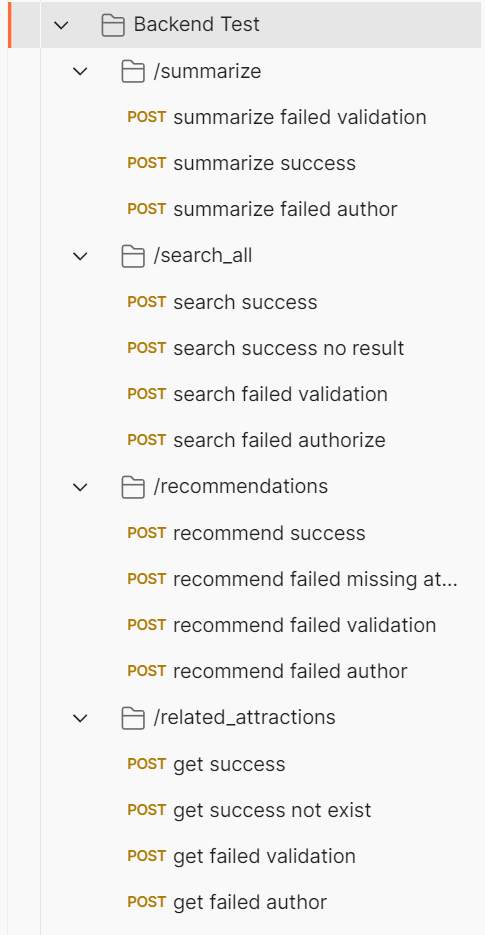
\includegraphics[width=0.6\textwidth]{figures/c4/api_test.png}
    \caption{Các API endpoint được kiểm thử với Postman.}
    \label{fig:postman}
\end{figure}
